\documentclass[ fontsize=11pt]{article}
\linespread{1.5}
% \usepackage[margin=2.5cm]{geometry}
\usepackage[margin=2.5cm, headheight=0pt, headsep=1cm]{geometry}
\usepackage{enumerate, fancyhdr, graphicx, amsmath, float, subcaption, textcomp, hyperref}


\title{Old School \tetris{} Meets Page Rank}
\author{Paul Chesnais (pmc85) \& Sam ``Sven'' Svenningsen (sjs382)}
\date{}

\def\tetris{Tetris\textsuperscript{\textregistered}}

\pagestyle{fancy}
\fancyhead{}
\lhead{pmc85 \& sjs382}
\chead{Old School \tetris{} Meets Machine Learning}
\rhead{\today}
\fancyfoot{}
\rfoot{\thepage}
\lfoot{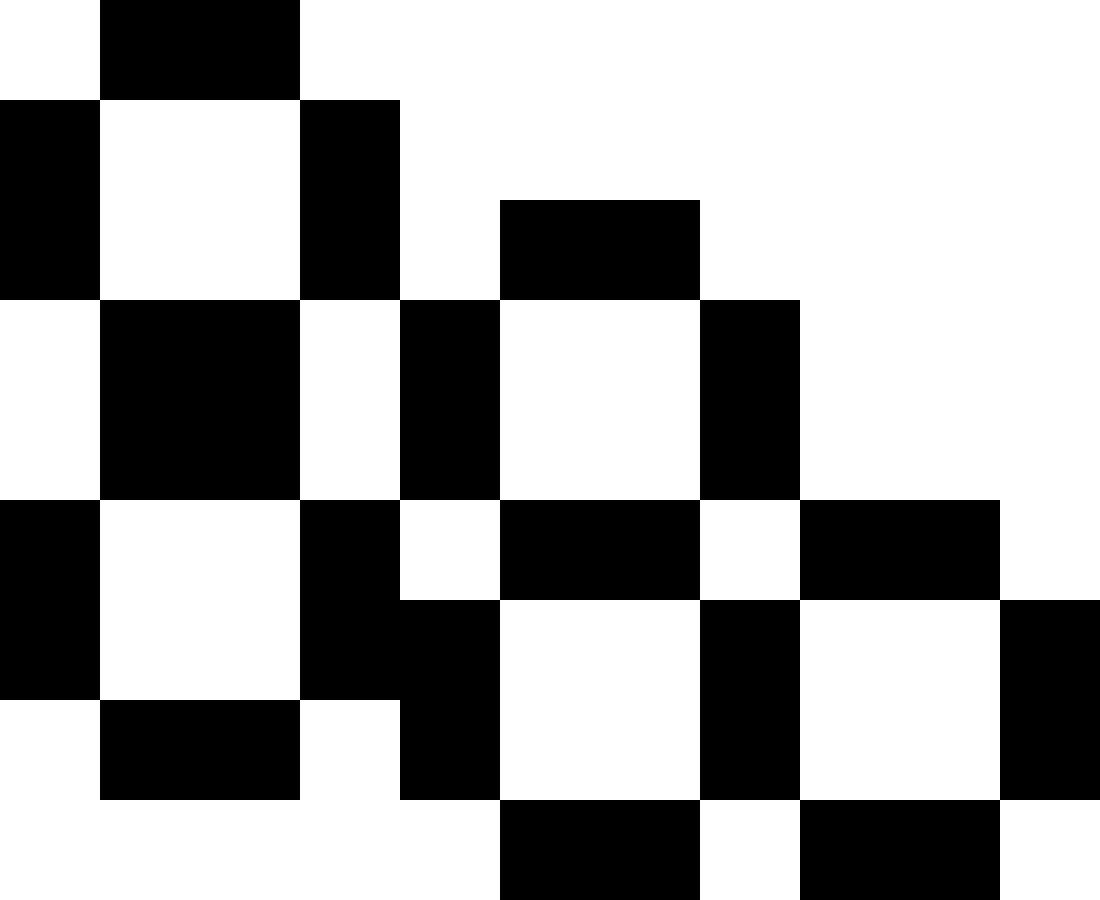
\includegraphics[height=20pt]{Logo}}
\renewcommand{\headrulewidth}{0.5pt}
\renewcommand{\footrulewidth}{0.5pt}

\usepackage{listings, color, times, textcomp, setspace}
\definecolor{Code}{rgb}{0,0,0}\definecolor{Decorators}{rgb}{0.5,0.5,0.5}\definecolor{Numbers}{rgb}{0.5,0,0}
\definecolor{MatchingBrackets}{rgb}{0.25,0.5,0.5}\definecolor{Keywords}{rgb}{0,0,1}\definecolor{self}{rgb}{0,0,0}
\definecolor{Strings}{rgb}{0,0.63,0}\definecolor{Comments}{rgb}{0,0.63,1}\definecolor{Backquotes}{rgb}{0,0,0}
\definecolor{Classname}{rgb}{0,0,0}\definecolor{FunctionName}{rgb}{0,0,0}\definecolor{Operators}{rgb}{0,0,0}
\definecolor{Background}{rgb}{0.98,0.98,0.98}

\lstdefinestyle{Scala}{
  backgroundcolor=\color{Background},basicstyle=\ttfamily\small\setstretch{1},breaklines=true,commentstyle=\color{Comments}\slshape,emph={self},emphstyle={\color{self}\slshape},frame=l,framexbottommargin=2em,framextopmargin=2em,keywordstyle={[2]\color{Decorators}\slshape},keywordstyle={\color{Keywords}\bfseries},morekeywords={abstract,case,catch,class,def,do,else,extends,false,final,finally,for,if,implicit,import,lazy,match,mixin,new,null,object,override,package,private,protected,requires,return,sealed,er,this,throw,trait,true,try,type,val,var,while,with,yield},otherkeywords={=>,<-,<\%,<:,>:,\#,@},sensitive=true,morecomment=[l]{//},morecomment=[n]{/*}{*/},morestring=[b]",morestring=[b]',morestring=[b]""",numbers=left,numbersep=1em,numberstyle=\footnotesize,showspaces=false,showstringspaces=false,showtabs=false,stringstyle=\color{Strings},tabsize=4,xleftmargin=1em,
}


\begin{document}
\maketitle
\thispagestyle{empty}
\section{Abstract}
\label{sec:abstract}

\par It has been shown that \tetris{}, the Russian tile-stacking puzzle video game, is NP-Complete \cite{tetrishard}. This project sought to try to approximate a solution to \tetris{} that plays well according to human standards. Evidently, no solutions can be perfect (assuming $P \neq NP$), but one can still try. The current algorithm approximates a solution by ranking the contour (the shape of the top of the stack) using a method akin to Google's PageRank algorithm, then choosing the sequence of Tetrominoes (\tetris{} pieces) that lead to the highest ranking stack.

\section{Getting computers to play \tetris{}}
\label{sec:getting_computers_to_play_tetris}

\subsection{An Introduction to the Game}
\label{sub:an_introduction_to_the_game}

\begin{figure}[h!]
  \centering
  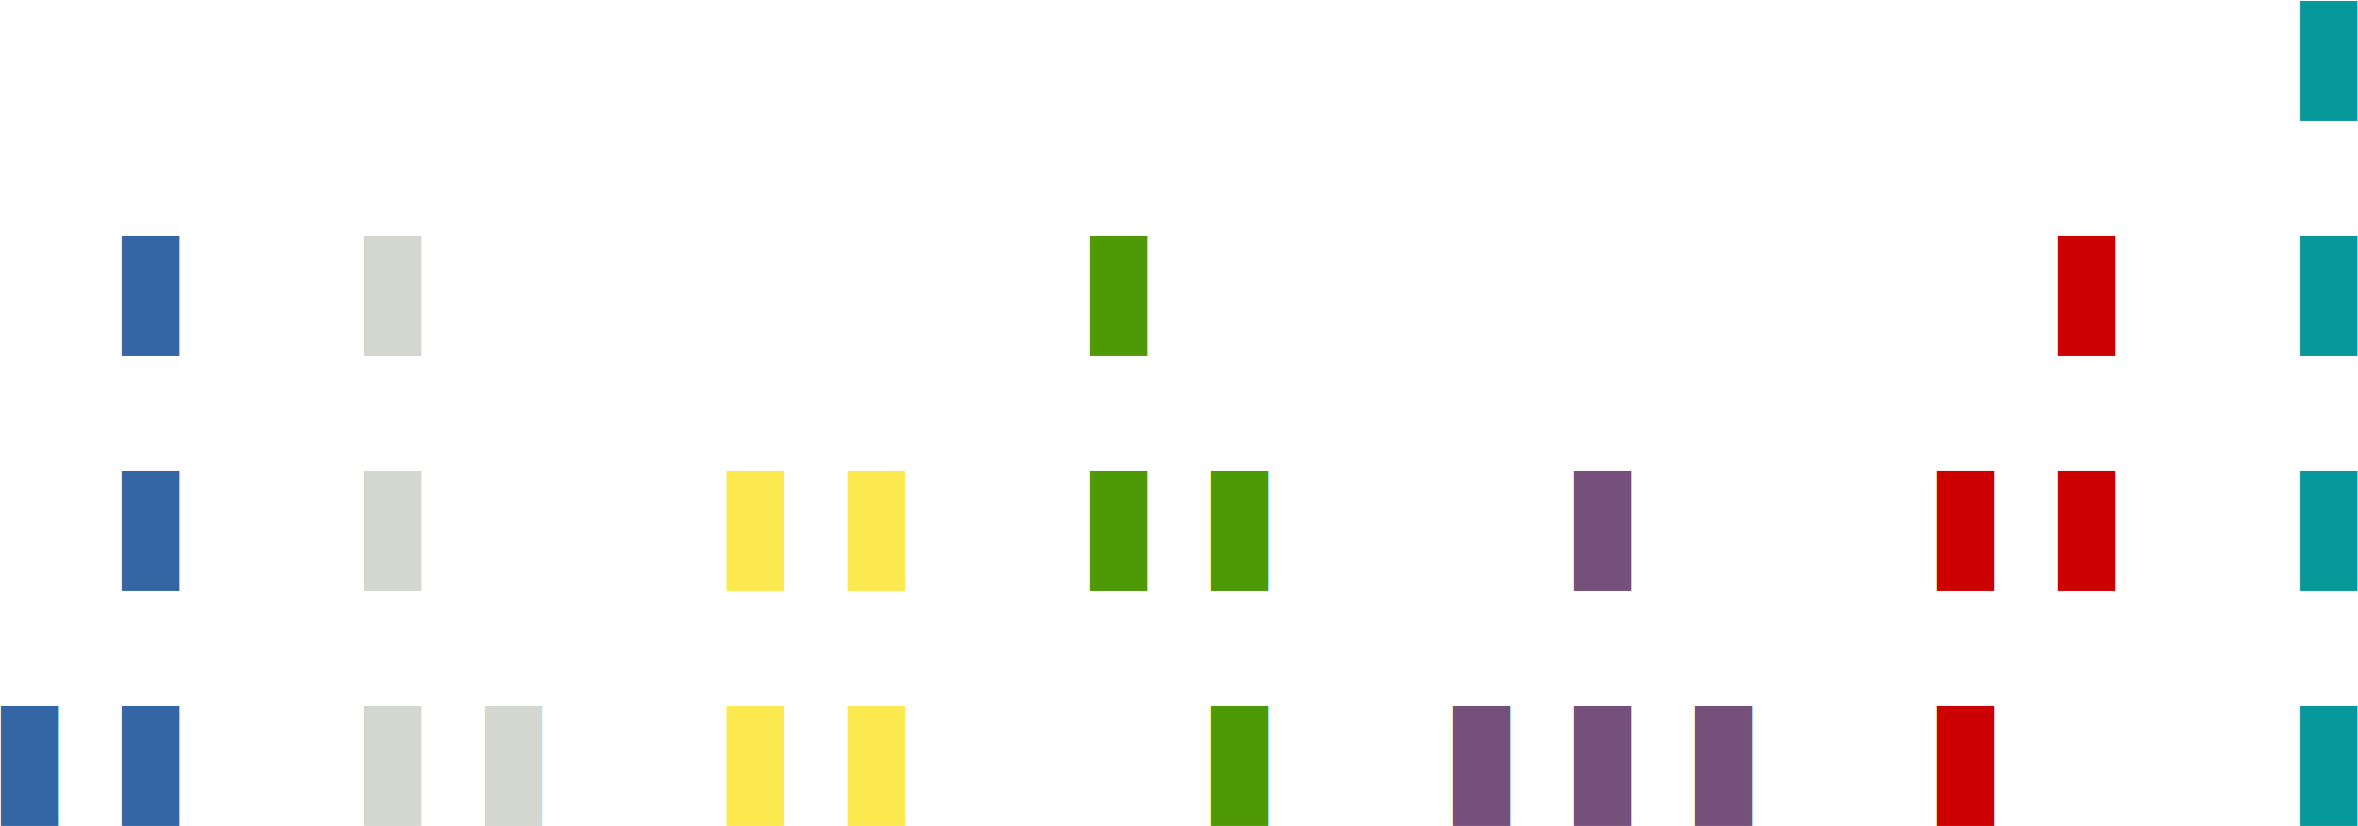
\includegraphics[width=0.4\textwidth, height=0.1\textwidth]{figures/pieces}
  \caption{The 7 tetrominoes J, L, O, S, T, Z and I }
  \label{fig:the_7_tetrominoes}
\end{figure}

\par The mechanics of \tetris{} are beautifully simple. The user begins with an game board, henceforth referred to as the ``stack'', 10 units wide and 20 units high. The user is then given a random sequence of the \tetris{} pieces, or ``tetrominoes'', shown in Figure~\ref{fig:the_7_tetrominoes}, to be placed on top of one another. Tetrominoes are each made up of 4 identical connected squares, and rotate by 90\textdegree clockwise or counterclockwise. When a tetromino is placed, it maintains its shape. In other words, it can create holes (see Figure~\ref{fig:placing_an_i_piece_to_clear_a_row}).
\par When a horizontal line is full, this line is removed. Every individual square above the cleared row then move directly downward $n$ vertical units, where $n$ is the number of row cleared. Figure~\ref{fig:placing_an_i_piece_to_clear_a_row} shows both the mechanic involved in clearing rows, and how poor placement of piece can create undesired holes. Here, the I piece was placed horizontally on top of the O, which blocks access to the three empty spaces below.
\par As time goes on, the amount of time the user has to place the piece decreases, making it difficult to keep up with, and to keep playing, the user must clear as many rows as possible to prevent the top of the stack from reaching height 20, otherwise, it's GAME OVER. The game is scored relative to how many rows were cleared by a single placement, and how frequently rows are cleared. The best score is achieved by using the I piece to clear 4 rows at once, and consecutive row clears multiply the score given (i.e. combos).

\begin{figure}[h!]
  \centering
  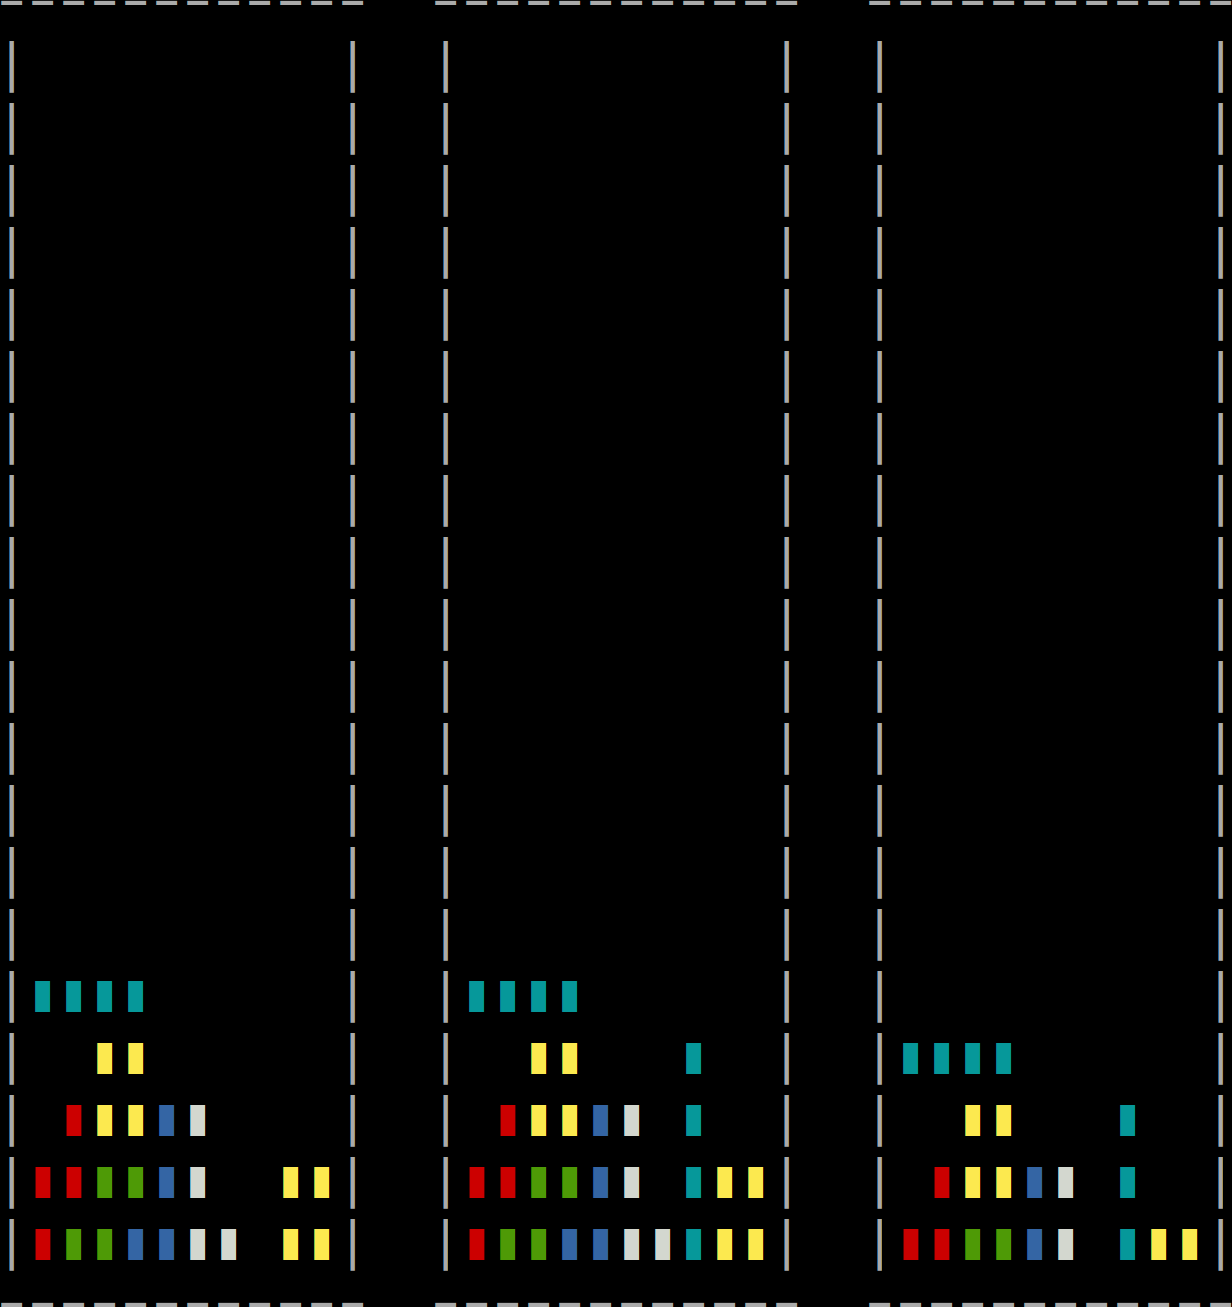
\includegraphics[width=0.6\textwidth, height=0.4\textwidth]{figures/rowclear-crop}
  \caption{Placing an I piece to clear a row}
  \label{fig:placing_an_i_piece_to_clear_a_row}
\end{figure}

\subsection{Representations}
\label{sub:representations}
\subsubsection{Tetrominoes}
\label{ssub:tetrominoes}

\par A simple, yet efficient efficient way to represent an single rotation of an individual tetromino is by keeping a list of two dimensional vectors representing the location of each square from the center of mass of the tetromino. Equation~\ref{eq:t_offsets} is an example of such a list for the T piece in the orientation shown in Figure~\ref{fig:the_7_tetrominoes}.
\begin{align}
  [(0,0), (-1, 0), (0, 1), (1, 0)]\label{eq:t_offsets}
\end{align}
With these lists and a given pair of coordinates $(x,y)$, finding the location of each square of a given tetromino only requires translating $(x,y)$ by each vector in the list.

\subsubsection{Arrays}
\label{ssub:array}
\par One way to represent a stack is with an array. In this case, the stack was represented as a $10\times 20$ two dimensional array, where each square in the theoretical stack maps to an element in the array. One square is represented as a tuple $(s,c)$ where $s$ is a boolean representing whether or not there exists a square in the stack at that location, and $c$ is the color of that square \footnote{Again, $c$ is only kept for graphical purposes and plays no role in the actual implementation}. It then becomes really easy to traverse the array to figure out whether a row is full.


\subsection{Relaxations}
\label{sub:relaxations}
\begin{description}
  \item[Scoring] The scoring scheme outlined above is unfortunately quite complex. Additionally, every implementation of \tetris{}
  \item[Timing]
\end{description}


\section{Motivation}
\label{sec:motivation}
The current


\section{Initial Attempts}
\label{sec:initial_attempts}

\subsection{MiniMax}
\par We tried to maximize the pieces placement in a way that would minimize the possible damage/maximize the least expected outcome of the next few pieces the \tetris{} board provides by using the MiniMax approach.
\subsubsection{Heuristic}
\par This lead us into the difficulty of grading boards on quality so that we could have a function to minimize over.

\par One thought would be to penalize boards that have holes or overhangs in them (i.e. pieces covering empty spaces), though penalize overhangs less since you can get around them sometimes.

\par The next obvious criteria was to give a max value to any board that has a \tetris{} (4 complete rows at once) and a lesser, but still high, score to any number of complete rows.

\par This leaves us an issue of all the boards with no obvious issues, and no obvious bonuses. We made a guess that having a more level board would be best (i.e. the distance between the lowest free spot and the highest tower you have is minimized).

\par An alternative to this is to make up as many features as possible and try to assign weights to them based on if they lead to failed games quickly (we'd have to play the game a bunch of times).

\par We weren't quite sure how to implement this though since we did not know how to weight each feature appropriately besides running it a million times over, which was too slow.

\subsubsection{Issues}
\par The size of the state space leads to some issues. There are about $10-40$ places to put a piece if you know which one it is (each piece has between 1 an 4 rotations and ~10 spots you can put it in), and $~190$ places you can put a piece each round for an unknown piece. So to do this n-places into the unknown piece space you have about $160*190^n$ pieces, which ends up being on the order of $10^{2n + 2}$ each round, even looking 4 pieces ahead into the unknown can take $10^{10}$ possible boards to check, which does not take a trivial amount of time.

\section{Challenges Faced}
\label{sec:challenges_faced}

\par Scala optimization


\section{Current Version}
\label{sec:current_version}



\section{Conclusion}
\label{sec:conclusion}

\newpage


\begin{thebibliography}{9}
\bibitem{tetrishard}
Erik D. Demaine, Susan Hohenberger, David Liben-Nowell
\textit{
Tetris is Hard, Even to Approximate}.
\\\href{https://arxiv.org/abs/cs/0210020}{arXiv:cs/0210020}

\end{thebibliography}

% \lstinputlisting[style=Scala]{../tetris/src/main/scala/tetris/Main.scala}

\end{document}
